% W ATCH THE U NOBSERVED : A S IMPLE A PPROACH TO PARALLELIZING MONTE CARLO TREE SEARCH
\setcounter{chapter}{3}

\chapter{Zrównoleglenie MCTS}
Celem zrównoleglenia MCTS jest przyśpieszenie wykonywania algorytmu poprzez lepsze wykorzystanie dostępnych zasobów sprzętowych przy jednoczesnym zachowaniu jakości podejmowanych decyzji. W tym rozdziale zostanie przedstawiony i rozwiązany problem z perspektywy CPU oraz GPU.

\hspace{3cm}

\section{Metoda batchowania danych}
Frameworki do pracy z sieciami neuronowymi, takie jak wykorzystywany PyTorch, są zoptymalizowane do pracy na partiach danych. Do teraz drzewo MCTS wykonywało się w pełni sekwencyjnie, czego skutkiem było przetwarzanie tylko jednej próbki danych przez sieć neuronową.

Ulepszona koncepcja polega na dodawaniu odpowiedniej liczby liści do bufora, tak aby można było je przetworzyć w jednej partii przez sieć neuronową. Po otrzymaniu wyników z sieci, drzewo jest aktualizowane poprzez wsteczną propagację. 

Głównym problemem jest brak aktualizacji statystyk drzewa w trakcie dodawania liści do bufora. Powoduje to, że podczas etapu selekcji algorytm PUCT nie ma aktualnych informacji o stanie drzewa przez co wybierana jest ta sama ścieżka. 

Można spróbować naiwnie rozwiązać ten problem poprzez blokowanie liści dodanych do bufora, wymuszając tym samym wybór innego liścia, aczkolwiek nie jest to optymalne rozwiązanie. Mimo takiego zabiegu wybierane są różne liście, jednakże posiadające tego samego rodzica, co można zaobserwować na rysunku 4.1. Taka metoda w praktyce jest szybsza, aczkolwiek znacznie mniej efektywana niż wersja sekwencyjna.

\newpage

\begin{figure}[h]
\centering
\includegraphics[width=0.8\textwidth]{images/mcts-naive-batch.png}
\caption{Naiwna metoda batchowania danych. Czerwone strzałki reprezentują wybraną najlepszą ścieżkę. Liść oznaczony numerem 6 został dodany do bufora i jest zablokowany. Na fioletowo została oznaczona ścieżka prowadząca do kolejnego liścia, który zostanie dodany do bufora.}
\end{figure}

\section{Fundament idealnego algorytmu równoległego}

W artykule "On effective parallelization of Monte Carlo Tree Search" \cite{EffectiveParallelMCTS} autorzy definiują warunki konieczne dla statystyk węzłów, które muszą zostać spełnione aby równoległe drzewo było nie tyle co szybsze, ale również tak samo skuteczne jak sekwencyjne:

\begin{equation}
\begin{aligned}
\overline{N}(s,a) &\ge N(s,a) + O(s,a) \\
\overline{G}(s,a) &:= \lvert \mathbb{E}[\overline{Q}(s,a)] - \mathbb{E}[Q_{m}^{\mathbb{A}_{\text{seq}}}(s,a)] \rvert = 0 \quad (m=N(s,a)+O(s,a))
\end{aligned}
\end{equation}

\noindent gdzie:
\begin{description}
  \item[$\overline{N}(s,a)$] - zmodyfikowana liczba odwiedzin akcji $a$ w stanie $s$
  \item[$N(s,a)$] - liczba odwiedzin akcji $a$ w stanie $s$
  \item[$O(s,a)$] - liczba liści w których trwają obliczenia dla akcji $a$ w stanie $s$
  \item[$G(s,a)$] - (ang. Gap) błąd estymacji wartości akcji $a$ w stanie $s$
  \item[$\overline{Q}(s,a)$] - zmodyfikowana wartość akcji $a$ w stanie $s$ w algorytmie równoległym
  \item[$Q_{m}^{\mathbb{A}_{\text{seq}}}(s,a)$] - wartość akcji $a$ w stanie $s$ w algorytmie sekwencyjnym po $m$ odwiedzinach
\end{description}

\vspace{0.5cm}

Powyższe warunki konieczne pokazują, że idealny algorytm równoległy musi w trakcie oczekiwania na wynik obliczeń, modyfikować tymczasowo statystyki węzłów. Powinny one być idealnie oszacowane, tak aby drzewo w każdej chwili czasowej dysponowało aktualnymi informacjami o swoim stanie. W przeciwnym razie, algorytm opierający swoje działanie na nieaktualnych wartościach dokonywałby nieoptymalnych wyborów węzłów, co można było zaobserwować na rysunku 4.1.

W praktyce spełnienie pierwszego warunku jest stosunkowo proste i zostało to rozwiązane przez implementacje WU-UCT, natomiast drugi warunek jest bardzo trudny do zrealizowania, gdyż wymaga przewidzenia wartości akcji.

\section{WU-UCT - Watch the Unobserved}
Metoda WU-UCT ma na celu spełnienie pierwszego z warunków koniecznych przedstawionych w równaniu (4.1). Wprowadza ona dodatkową zmienną $O(s,a)$, która przechowuje informację o liczbie liści, dla których trwają obecnie obliczenia w akcji $a$ w stanie $s$. W momencie wyboru liścia, wartość tej zmiennej jest inkrementowana dla każdego węzła na wybranej ścieżce. Po otrzymaniu wyniku, jest ona dekrementowana w trakcie wstecznej propagacji.

Zmienna $O(s,a)$ jest wykorzystywana w zmodyfikowanym wzorze PUCT do uzupełnienia informacji o liczbie odwiedzin węzła. W efekcie algorytm dynamicznie koryguje wartość eksploracji w zależności od liczby trwających obliczeń węzłów potomnych. Wyższa wartość $O(s,a)$ skutkuje mniejszą wartością eksploracji. Pozwala to na unikanie podążania za ścieżkami, w których trwają już obliczenia, skupiając się na eksploracji innych części drzewa.

Mechanizm blokowania przedstawiony w podrozdziale 4.1, pełni teraz tylko rolę zabezpieczenia. Zapewnia on, że do bufora nie zostanie dodany ten sam liść. W najgorszym przypadku zostanie dodany najlepszy liść tego samego rodzica, który nie znajduje się w buforze.

\vspace{1cm}

\begin{equation}
\operatorname{WU-UCT}(s,a) \,=\, \widehat{Q}(s,a) \, + \, c_{\mathrm{puct}}\, P(s,a)\, \frac{\sqrt{(\sum_{b} N(s,b)) + O_s}}{(1 + N(s,a)) + O_s}\, ,
\end{equation}
\noindent gdzie:
\begin{description}
  \item[$\widehat{Q}$] - średnia wartość akcji $a$ w stanie $s$
  \item[$N(s)$] - liczba odwiedzin stanu $s$
  \item[$N(s,a)$] - liczba odwiedzeń akcji $a$ w stanie $s$
  \item[$\sum_{b} N(s,b)$] - suma odwiedzin wszystkich akcji w stanie $s$
  \item[$P(s,a)$] - prawdopodobieństwo wyboru akcji $a$ w stanie $s$ zwracane przez sieć neuronową
  \item[$c_{puct}$] - współczynnik eksploracji
  \item[$O_s$] - suma trwających obliczeń węzłów potomnych stanu $s$
\end{description}

\begin{figure}[h]
\centering
\includegraphics[width=0.8\textwidth]{images/WU-UCT.png}
\caption{WU-UCT. Czerwona strzałka przedstawia najlepszą ścieżkę, natomiast fioletowa przedstawia ścieżkę do kolejnego liścia dodawanego do bufora}
\end{figure}

\newpage

Na poniższym listingu można zauważyć bardzo dużą różnicę między naiwnym blokowaniem wybranych liści, a wykorzystaniem metody WU-UCT. Dzięki spełnieniu pierwszego warunku koniecznego, algorytm WU-UCT skuteczniej eksploruje drzewo, wybierając liście z różnych części drzewa, a nie tylko z tej samej gałęzi.

\begin{lstlisting}[
    language=Python,
    caption=Adresy rodziców 8 liści znajdujących się w buforze,
    inputencoding=utf8,
    basicstyle=\ttfamily\footnotesize,
    backgroundcolor=\color{gray!10},
    frame=single,
    showspaces=false,
    showstringspaces=false,
    numbers=none
]
Blokowanie:
0x705d41c78440
0x705d41c78440
0x705d41c78440
0x705d41c78440
0x705d41c78440
0x705d41c78440
0x705d41c78440
0x705d41c78440

WU-UCT:
0x7a5e5d1e1be0
0x7a5e5d1e38f0
0x7a5e5d1f1640
0x7a5e5d1f3350
0x7a5e5d0010a0
0x7a5e5d002db0
0x7a5e5d00cb00
0x7a5e5d00e810
\end{lstlisting}

\newpage

\section{Wady batchowania danych}
Przedstawione podejście batchowania danych rozwiązuje problem nieoptymalnego wykorzystania GPU. Jednakże po rozwiązaniu problemu narodziły się kolejne.

Algorytm WU-UCT spełnia tylko pierwszy z warunków koniecznych przedstawionych w równaniu (4.1). Drugi warunek mówiący o idealnym oszacowaniu wartości akcji nadal nie jest spełniony. W praktyce oznacza to, że drzewo MCTS nie posiada idealnych informacji o swoim stanie, przez co wraz ze wzrostem rozmiaru bufora zwiększa się bias algorytmu.

Kolejnym występującym problemem jest sam język Python. Jest on językiem interpretowanym, przez co niespodziewanym wąskim gardłem stały się najprostsze operacje utrzymujące drzewo. Szczególnie jest to widoczne przy etapie ekspansji, gdzie czas wykonania wynosi $O(n * m)$, gdzie $n$ to wielkość bufora, a $m$ to liczba możliwych ruchów z danego stanu (średnio ok 45). Taka pętla jest znacznie wolniejsza niż sama sieć neuronowa, przez co zwiększanie rozmiaru bufora nie przekłada się na duży wzrost szybkości wykonania.

W efekcie powyższych problemów, zwiększanie rozmiaru bufora nie tylko nie przekłada się na widoczną poprawę czasu wykonania, ale również pogarsza się jakość podejmowanych decyzji.

\begin{figure}[!h]
\centering
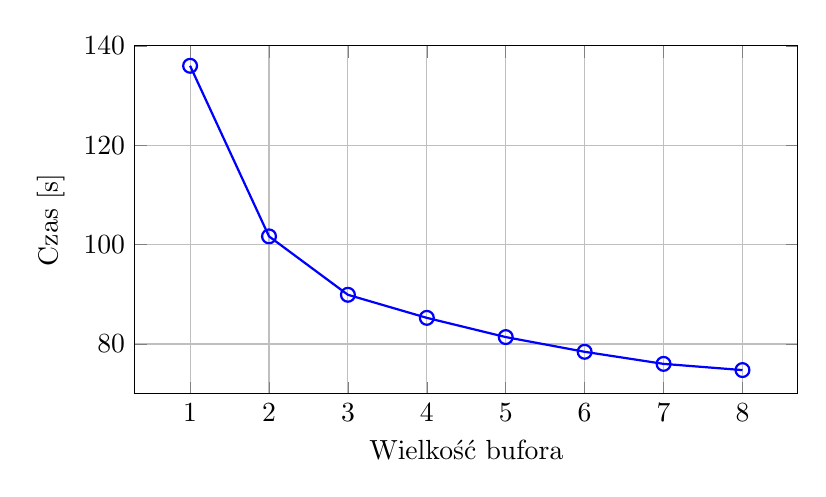
\begin{tikzpicture}
  \begin{axis}[
      width=10cm,
      height=6cm,
      grid=both,
      xlabel={Wielkość bufora},
      ylabel={Czas [s]},
      xtick={1,2,3,4,5,6,7,8},
      ymin=70,
      ymax=140,
      ymajorgrids=true,
      xmajorgrids=true,
      legend style={at={(0.02,0.98)},anchor=north west,font=\small},
      mark size=2.5pt
  ]
    \addplot+[blue, thick, mark=o] coordinates {
      (1,135.98)
      (2,101.66)
      (3,89.9)
      (4,85.26)
      (5,81.39)
      (6,78.43)
      (7,76.0)
      (8,74.75)
    };
  \end{axis}
\end{tikzpicture}
\caption{Wpływ wielkości bufora na czas wykonania 6000 iteracji}
\label{fig:metric-iteracje}
\end{figure}

Testy wydajnościowe przedstawione na wykresie zostały przeprowadzone na procesorze i7-11800H oraz GPU RTX 3060. Na wykresie 4.3 można zaobserwować, że wraz ze wzrostem wielkości bufora, różnica czasu wykonania maleje. 

Jako optymalną wartość rozmiaru bufora wybrano 2, gdyż daje ona bardzo duży zysk czasowy, a jednocześnie brak spełenia drugiego warunku koniecznego nie ma dużego wypływu na jakość podejmowanych decyzji. Na wykresie 4.4 można zauważyć, że używając tego samogo czasu na oblieczenie ruchu, algorytm z buforem o rozmiarze 2 osiąga przewagę nad sekwencyjną wersją.
\begin{figure}[h]
\centering
\includegraphics[width=0.55\textwidth]{images/buffor-comp.png}
\caption{Rozgrywka między sekwencyjnym MCTS a MCTS z buforem o rozmiarze 2 przy tym samym czasie wykonania. Rozgrywka została oceniona przez silnik Stockfish.}
\end{figure}


\newpage

\section{Wieloprocesowy MCTS}
Do tej pory opisywane metody skupiały się na większym wykorzystaniu GPU. Jednakże dużym ograniczeniem stanowią operacje na drzewie wykonywane przez CPU. Dzisiejsze procesory posiadają stosunkowo dużą liczbę rdzeni, które można wykorzystać do przyśpieszenia obliczeń. 

Do zrównoleglenia algorytmu zostały użyte wszystkie omówione wcześniej techniki, takie jak batchowanie danych z buforem o rozmiarze 2 oraz WU-UCT. Działanie samej równoległości opiera się na metodzie tree parallelization, gdzie jedno drzewo jest współdzielone między wszystkimi workerami. 

\subsection{Struktura drzewa}
Język Python jest językiem jednowątkowym przez co koniecznym było użycie wieloprocesowości. Głównym problemem w takim podejściu jest brak współdzielonej pamięci programu między procesami. Z tego powodu konieczne było wydzielenie fragmentu pamięci dynamicznej do przechowywania współdzielonej struktury drzewa. Z poziomu Pythona ma ona postać zwykłych bajtów, przez co możliwe są tylko dwa rozwiązania przechowywania obiektowej struktury: spłaszczenie, lub użycie serializacji wraz z deserializacją. Z oczywistych względów wydajnościowych jak i prostoty implementacji została wybrana pierwsza metoda.

Ze względu na fakt, że używając współdzielonaj pamięci jest tylko dostęp do bloku bajtów, spłaszczona struktura musi być przechowywana w tablicy. Ogólne działanie drzewa jest oparte na podobnej zasadzie co wersja obiektowa. Z taką różnicą, że zamiast operować na referencjach, operujemy na indeksach tablicy. Każdy węzeł zawiera informacje o id rodzicu oraz dzieci. Statystyki drzewa są przechowywane identycznie jak w wersji obiektowej. Różnica pojawia się tylko przy stanie gry, czyli planszy. Zamiast serializować i deserializować obiekt BoardPlus, plansza jest przechowywana w znacznie bardziej kompaktowej formie, jako tablica charów oraz zmiennej bool. Opisują one kolejno stan planszy w formacie FEN oraz perspektywę rozgrywki. Format FEN był opisywany w pierwszym rozdziale.

Każda zmienna została dobrana pod kątem minimalizacji zużycia pamięci. Przykładowo liczba odwiedzin jest przechowywana jako 16 bitowa liczba całkowita bez znaku, gdyż w praktyce nie zdarza się aby liczba odwiedzin przekroczyła 65535 oraz była ujemna. Dodatkowo ze względu na użycie tablic, wszystkie ich rozmiary są ustalane przed rezerwacją pamięci. Rozmiar drzewa jest obliczany na podstawie wzoru 4.3, gdzie brana jest pod uwagę maksymalna liczba dzieci na węzeł oraz liczba symulacji. Maksymalna liczba dzieci jest stała i wynosi 100, co jest wartością bardzo bezpieczną, gdyż średnia liczba możliwych ruchów w szachach wynosi około 45.

\vspace{0.5cm}

\begin{equation}
\operatorname{treeSize} \,=\, \operatorname{maxChildrenPerNode} \times \operatorname{simNumber} + 1
\end{equation}

\begin{lstlisting}[
    language=Python,
    caption=Struktura tablicy przechowującej drzewo MCTS w pamięci współdzielonej,
    inputencoding=utf8,
    basicstyle=\ttfamily\footnotesize,
    backgroundcolor=\color{gray!10},
    frame=single,
    showspaces=false,
    showstringspaces=false,
    numbers=none
]
tree_dtype = np.dtype([
    # -1 for root
    ('parent_id', np.int32),
    # avg max children per node is ~(30-55)
    ('children', np.uint32, MAX_CHILDREN_PER_NODE), 
    ('children_count', np.uint8),
    ('fen', 'S100'),
    ('changed_perspective', np.bool_),
    ('move_id', np.int16), # -1 for root
    ('total_visit', np.uint16),
    ('total_reward', np.float32),
    ('prior', np.float32),
    ('unobserved_samples', np.uint32),
    ('is_locked', np.bool_),
    # result for terminated states. 2 for not terminated
    ('result', np.int8)
])
\end{lstlisting}

\vspace{0.5cm}

Powyższa struktura uwzględnia również zmienną result przechowującą wynik gry dla zakończonych stanów. Wartość ta jest dodawana w momencie ekspancji. Pozwala to uniknąć niepotrzebnej kolejnej zamiany fen na obiekt klasy BoardPlus bezpośrednio po selekcji.

\vspace{2cm}

\begin{figure}[h]
\centering
\includegraphics[width=1\textwidth]{images/tree_structure.png}
\caption{Struktura drzewa w pamięci współdzielonej}
\end{figure}

\newpage

\subsection{Działanie wieloprocesowego MCTS}
Ostatnim wyzwaniem było zaprojektowanie procesów wykonawczych wraz z ich synchronizacją, gdzie każdy z nich ma za zadnie wykonanie takiej samej liczby symulacji. Trzeba wziąć pod uwagę fakt, że wszystkie operacje będą odbywały się na jednym drzewie. Szczególnie jest to problematyczne w początkowej fazie, gdzie przez dostępność małego zbioru liści, może dojść do sytuacji gdzie wiele procesów będzie podążało tą samą ścieżką osiągając ten sam liść.

Bardzo dobrze ilustruje to przypadek widoczny na rysunku 4.6, gdzie algorytm po inicjalizacji zaczyna wykonywać pierwszą selekcję zaczynając od korzenia. Naturalnie jest tylko jeden korzeń w drzwie, więc trzeba wówczas zapewnić że tylko jeden proces będzie mógł go rozwinąć, a pozostałe będą musiały czekać. Obsługa takiego przypadku jest zaprezentowana na rysunku 4.7, gdzie algorytm od razu sprawdza czy są dostępne liście. Jeżeli nie, to czeka, albo przetwarza swój bufor niezależnie od rozmiaru. Wywołanie przetwarzania bufora w takim przypadku ma na celu uniknięcie sytuacji, gdzie procesy same się blokują czekając na odblokowanie liści w buforach.

\begin{figure}[h]
\centering
\includegraphics[width=0.6\textwidth]{images/waiting-proc.png}
\caption{Procesy oczekujące na dostępne liście}
\end{figure}


Następnym bardzo ważnym aspektem w równoległości jest integralność danych. Zapewniona jest ona przez użycie dwóch blokad. Oznaczone odpowiednio jasnobrązowym oraz zielonym kolorem na rysunku 4.7 i 4.8. Widoczny duży jasnobrązowy blok odpowiada za zapewnienie atomowości operacji wyboru liścia. Dzięki temu tylko jeden proces może wykonać kolejno: wybór liścia, aktualizacje tymczasowej statystyki oraz zablokowanie. Unikamy w ten sposób sytuacji, gdzie dwa procesy przetwarzają ten sam liść.
\begin{figure}[h]
\centering
\includegraphics[width=1\textwidth]{images/multiproc-mcts.png}
\caption{Schemat procesu w wieloprocesowym MCTS}
\end{figure}

\newpage

Na rysunku 4.7 jest przedstawiona również druga blokada. Odpowiada ona za integralność zmiennej przechowującej ostatni zapisany indeks w tablicy drzewa. Jest to istotne podczas ekspansji, gdzie nowy węzeł jest tworzony na indeksie wskazywanym przez tę zmienną.
\begin{figure}[h]
\centering
\includegraphics[width=1\textwidth]{images/buffor-schematic.png}
\caption{Schemat przetwarzania bufora}
\end{figure}

\section*{Ewaluacja MCTS}
Najbardziej obiektywnym sposobem oceny działania całego algorytmu szachowego jest porównanie go z innym. Wybrany został Stockfish ze względu na jego popularność oraz wsparcie biblioteki \textit{chess} ułatwiającej integrację.

Porównanie polega na rozegraniu podanej liczby partii pomiędzy dwoma silnikami. Białe figury są reprezentowane przez Stockfish, a czarne przez opisywany model. Główną miarą oceny jest przeżywalność, czyli liczba ruchów w danej partii. Dodatkowo w celu uzyskania bardziej szczegółowych danych, stockfish w każdej rundzie podaje ocenę pozycji dla czarnych figur. Mieści się ona w przedziale od -1000 do 1000, gdzie skrajne wartości oznaczają mat.
W pliku konfiguracyjnym użytkownik za pomocą wartości \textit{stockfish\_gen\_moves} może ustawić ilość generowanych ruchów przez Stockfish w danej turze. Spośród nich jest losowany ostateczny ruch. Taki mechanizm pozwala na znaczne obniżenie poziomu trudności silnika. Było to szczególnie bardzo istotne w początkowej fazie rozwoju modelu, gdzie jego skuteczność była niska. Obecnie ze względu na dobrą jakość implementowanego algorytmu, wartość ta jest ustawiona na 1, co oznacza że Stockfish nie jest osłabiany.

Na wykresach porównawczych jest również uwzględniony wynik losowego modelu, który w każdej turze wybiera losowy (legalny) ruch. Pełni on rolę poziomu odniesienia.

\begin{figure}[h]
\centering
\includegraphics[width=0.6\textwidth]{images/stockfish.png}
\caption{Wykres przeżywalności modelu względem Stockfish}
\end{figure}
